\noindent\textbf{Algebra II Final Examination \hspace{\fill} Luis Berlioz}
\problem{1}
Indeed every Euclidean domain is a PID. This is because a Euclidean ring is a  principal ideal ring with identity; additionally assuming our ring is an integral domain implies we get a PID.

On the other hand, it is not true that any PID is a Euclidean domain. A counter example of this is the ring $R=\ZZ[\theta]$ where $\theta=(1+\sqrt{-19})/2$. To show $R$ is not a Euclidean domain we start by pointing out that:
\[R=\{a+b\theta\from a,b\in\ZZ\}\]
The reason for this is that $\theta$ satisfies the polynomial $x^2-x+5\in \ZZ[x]$. This implies that any monomial of order greater than 1 can be reduced to a linear combination of just 1 and $\theta$ using the identity $\theta^2=\theta-5$.

To prove that the only units are $\pm 1$, observe that if $a+b\theta\in R$ is a unit then:
\begin{align*}
   1 =(a+b\theta)(a+b\bar\theta) &= a^2+2abRe\theta +b^2\theta\bar\theta\\
                           &= a^2+2abRe\theta +b^2(\theta-5)\\
                           &= a^2+5b^2+2ab\,Re\theta
\end{align*}
In the case where $b=0$ we get $a^2=1$, for $b\neq 0$ parameterizing for $b$ and solving for $a$ gives no more integer solutions.

Next we show that an Euclidean function is impossible to define in $R$. Suppose for the sake of contradiction that such a function namely $\phi$ exists. Since $\phi$ ranges in the natural numbers, it has a minimum say $x\in R$. Given that for any $y\in R$ not a unit there exists $q,r\in R$ such that $y=qx+r$.  Observe that $\phi(x)> \phi(r)$ is not an option and thus we get $y= q\, x$. Since $x$ is not a unit, we conclude that the ideal $(x)$ contains everything but the units, thus $R/(x)$ has 2 of 3 elements.

In the case of $R/(x)$ containing 2 elements then $\alpha^2-\alpha+5=5$ so no root is feasible. Next, if $R/(x)$ has three elements then:
$$\alpha^2-\alpha+5= 6-\alpha = -\alpha$$
And the only solution is $\alpha=0$ which contradicts that $R$ properly contains $\ZZ$. Therefore we conclude that a Euclidean function is impossible over $R$.

Last but no least, observe that $R$ is a PID. This is given by Theorem III.2.16 since the quotient of any ideal $P$ and $R$ is a integral domain as we showed above. 

\problem{2}
The polynomial $(x^3-1)(x-2)$ has $[K(\alpha,\beta,\gamma):K]=3$. To show this last assertion, let $\omega= -\frac 12 +i\frac{\sqrt 3}{2}$ be the first complex cubic root of unity, letting $u_1=1,\ u_2=\omega,\ u_3=\omega^2,\ u_4=2$ then:
\begin{gather*}
    \alpha = u_1u_2 + u_3u_4 = -\frac{1}{2} i \, \sqrt{3} - \frac{3}{2}\\
    \beta = u_1u_3 + u_2u_4 = \frac{1}{2} i \, \sqrt{3} - \frac{3}{2}\\
    \gamma = u_1u_4 + u_2u_3 =3
\end{gather*}
And has resolvent cubic:
$$(x-\alpha)(x-\beta)(x-\gamma)= x^3 - 6x - 9$$
The key is that $\alpha=1+\omega^2$ and $\beta=\omega-1$ and thus $[K(\alpha,\beta,\gamma):K]=3$ as claimed. 

By trial and error and using Theorem V.4.12 the following polynomial with exactly 5 real roots. 
$$x^7-3\cdot10^{4}x^3 + 3\cdot 10^5x- 3\cdot 10^5$$
By the rule of signs and using the graph shown below, it has 3 positive 2 negative roots. Also it is of order 7 and irreducible by Eisenstein with prime 3.
    \begin{figure}[h]
\begin{center}
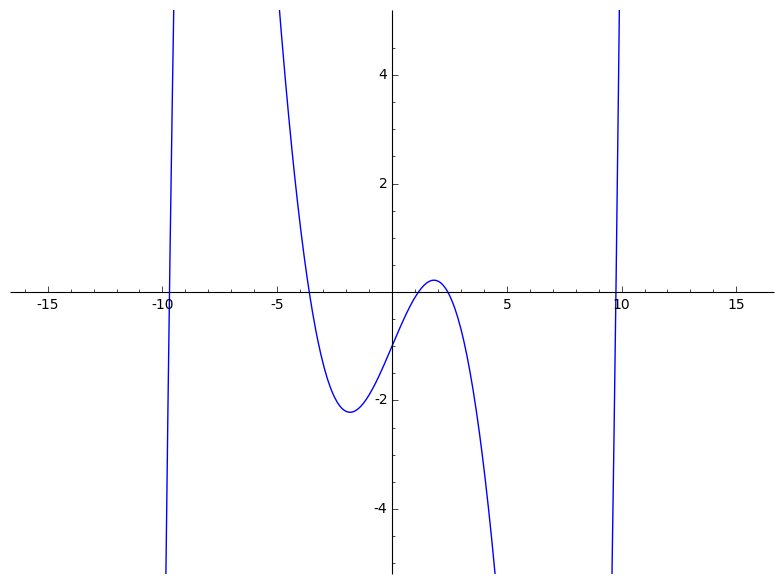
\includegraphics[width=0.5\textwidth]{sage0.png}
\caption{Graph of the polynomial $10^{-5}x^7-30^{-1}x^3 + 3x- 3$}
\end{center}
\end{figure}

\problem{3}
Let $\theta \from \hom_S(B,C)\otimes_R B \to C$ defined as:
$$\theta (h\otimes_R b)= h(b)$$
Where $h\in \hom_S(B,C)$ and $b\in B$. Observe that the tensor product  $\hom_S(B,C) \otimes_R B$ makes sense because:
$$b \otimes_R(rb) = (h\, r) \otimes_ R b$$
And $h\,r$ is well-defined whenever it is for the argument of this morphism by setting it to be $h\, r =h \circ \pi_r$. And $\pi_r$ is the premultiplication morphism $\pi_r(b)=r\, b$.

Likewise, $\theta$ is a well-defined right $S-$module and group morphism, to wit:
$$\theta((h \otimes_ R b)s)=\theta(h \otimes_ R (b\, s))=h(b\, s)= h(b)s$$
And for an also arbitrary $b'\in B$:
$$\theta(h \otimes_ R (b+b'))=\theta(h \otimes_ R b+ h \otimes_ R b')=h(b+b')=h(b)+h(b')$$
Idem for the case of $(h+h')  \otimes_ R b$.

On the other hand, now take $\lambda \from A \to \hom_S(B,A\otimes_R B)$\footnote{The ``misprint''  is that $R$ appears here as the base ring, but $S$ is the best choice in this case.} defined as: $\lambda (a) = h_a\in \hom_S(B,A\otimes_R B)$ defined for all $a\in A$ and $b\in B$ as: 
$$h_a(b) = a \otimes_R b $$
Notice that $\lambda$ is a well-defined right $R-$module homomorphism since $\lambda(a\,r) = h_{ra}$ and:
$$h_{a\,r}(b) = (a\, r) \otimes_ R b = a \otimes_ R (r\,b)= h_a(r\, b) = h_ar(b)$$
Since this is the case for any $b\in B$ then $\lambda(ar)= h_a r= \lambda(a)r$. To show that $\lambda$ is a group morphism requires of  an identical proof.

\problem{4}
$K=\ZZ_2(x)$ is a field in which the element $x$ is prime. This is because assuming that $x$ is reducible would imply it is algebraic over $\ZZ_2$. Using this result, the polynomial $y^2- x\in \ZZ_2(x)[y]$ turns out to be irreducible by the Eisenstein's criterion. Moreover, the formal derivative of $y^2-x$ is zero and thus not separable.

Next we argue that all irreducible polynomials in a finite field are separable. Consider a finite field $K$ with characteristic $p$. Assume for the sake of contradiction that $f\in K[x]$ is an irreducible polynomial of positive degree that is not separable. Then $f'=0$ and this means that $f$ can be written as a polynomial in $x^p$. 

To see the last assertion it is enough to work on a monomial $x^k$. If it is not zero, and its derivative is, then it must be the case that $k\, x^{k}=0\, x$, equivalently, $k\equiv 0 \mod p$.

By Fermat's little theorem:
$$f(x) = a_n x^{p\,n}+\ldots + a_0 = (a_n+\ldots +a_1)x +a_0$$
And we get the contradicting conclusion that a linear polynomial is irreducible.
\problem{5}
From Theorem V.5.3 (almost verbatim). In the case $G\neq \{1\}$, then $G$ has to be a finitely generated Abelian group. Using the representation theorem for these, we get that any element in $G$ is a root of unity and thus cyclic.

\problem{6}
Let $\phi \from A\to B$ be a monomorphism. The induced morphims of $\phi$ is defined for all $f\in \hom(B,\QQ/\ZZ)$ as: 
$$\theta f= id\circ f\circ \phi$$
In specific if we look at $A,B$ as $\ZZ-$modules,  $\phi$ becomes a $\ZZ-$module homomorphism that is injective thus the following sequence is split exact:
$$0\to A \xrightarrow \phi B \to B \to 0$$
By Proposition IV.4.4 this is equivalent to:
$$0\to \hom(B,\QQ/\ZZ) \to \hom(B,\QQ/\ZZ) \xrightarrow \theta \hom(A,\QQ/\ZZ) \to 0$$
Being an exact sequence of Abelian groups.

